

\begin{figure}[H]
\centering
\resizebox{\textwidth}{!}{%
    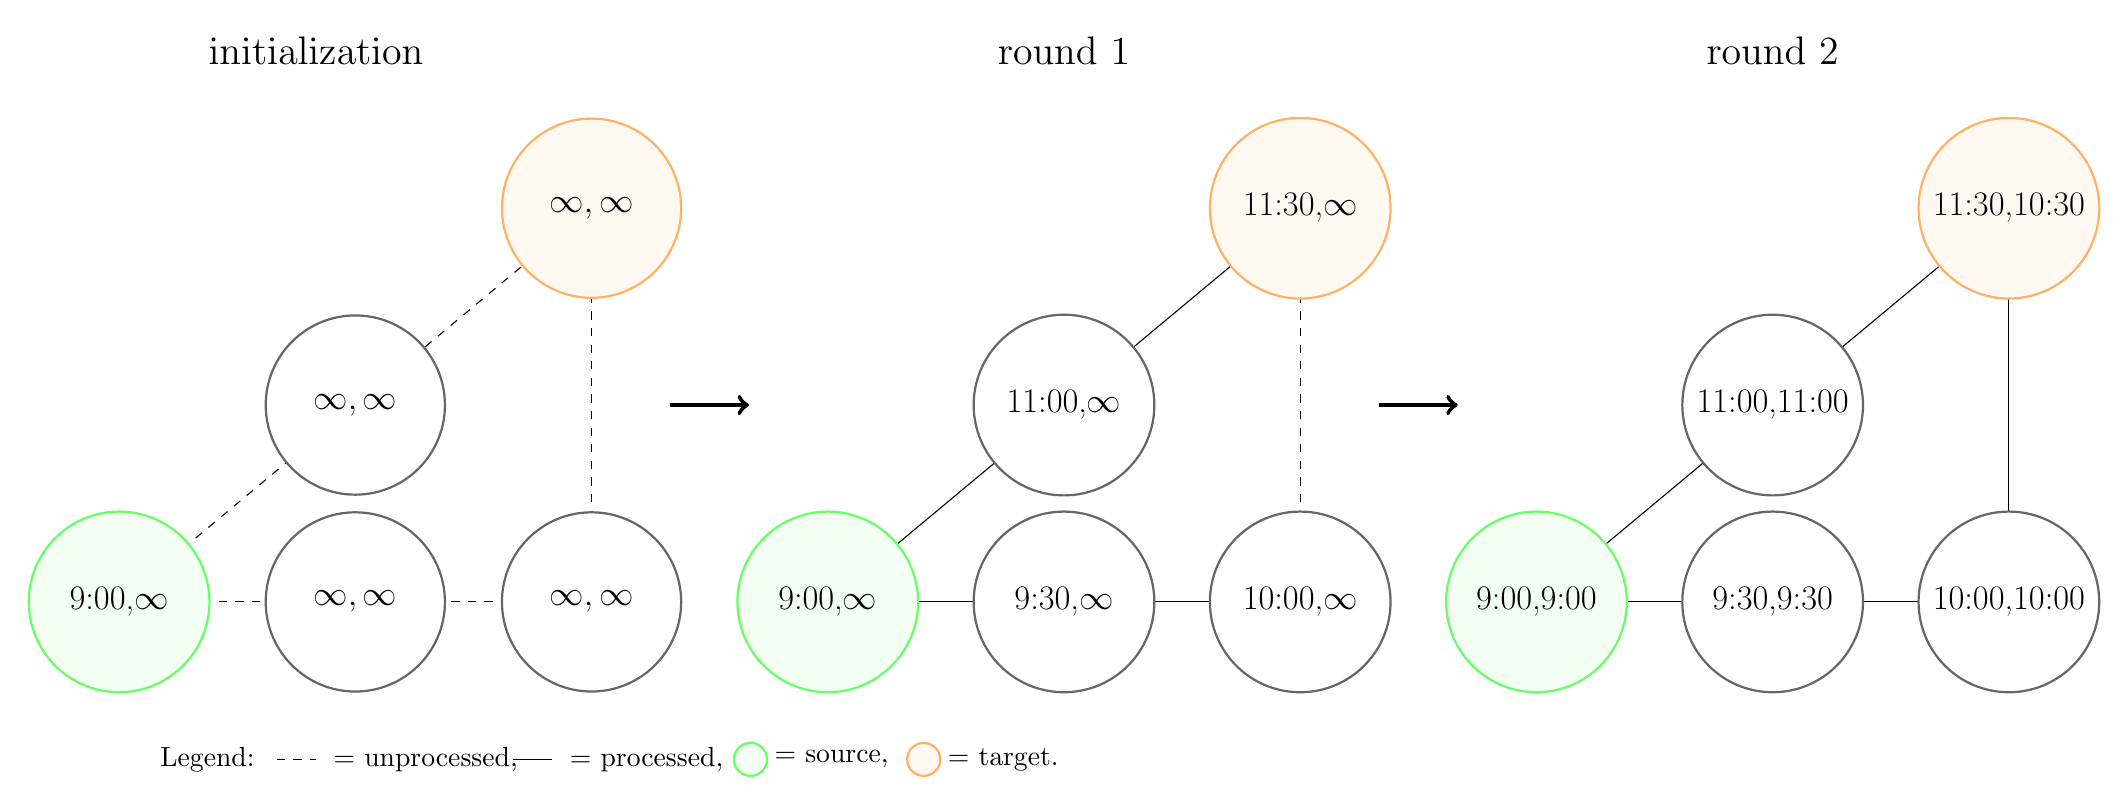
\begin{tikzpicture}[
roundnode/.style={circle, thick, minimum size=7mm, text width=3.5cm,align = center,scale=0.6,font=\huge},
green/.style={draw=green!60, fill=green!5},
orange/.style={draw=orange!60, fill=orange!5},
white/.style={draw=black!60, fill=white},
]
    \draw (0.4,-2) node[right=0] {Legend:};
    \draw [dashed](2,-2) -- (2.5,-2);
    \draw (2.6,-2) node[right=0] {= unprocessed,};
    \draw [](5,-2) -- (5.5,-2);
    \draw (5.6,-2) node[right=0] {= processed,};
    \draw (7.8,-2) node[roundnode,text width=0.4cm,green,right=0] {};
    \draw (8.2,-2) node[right=0] {= source,};
    \draw (10,-2) node[roundnode,text width=0.4cm,orange,right=0] {};
    \draw (10.4,-2) node[right=0] {= target.};
    
    \draw [dashed](0,0) -- (6,0);
    \draw [](9,0) -- (15,0);
    \draw [](18,0) -- (24,0);
    

    \draw [dashed](6,0) -- (6,5);
    \draw [dashed](15,0) -- (15,5);
    \draw [](24,0) -- (24,5);
    

    \draw [dashed](0,0) -- (6,5);
    \draw [](9,0) -- (15,5);
    \draw [](18,0) -- (24,5);
    
    \draw[->, ultra thick] (7,2.5) -- (8,2.5);
    \draw[->, ultra thick] (16,2.5) -- (17,2.5);
    
    \draw (0,0) node[roundnode,green] {9:00,$\infty$};
    \draw (3,0) node[roundnode,white] {$\infty,\infty$};
    \draw (6,0) node[roundnode,white] {$\infty,\infty$};
    \draw (3,2.5) node[roundnode,white] {$\infty,\infty$};
    \draw (6,5) node[roundnode,orange] {$\infty,\infty$};

    
    \draw (9,0) node[roundnode,green] {9:00,$\infty$};
    \draw (12,0) node[roundnode,white] {9:30,$\infty$};
    \draw (15,0) node[roundnode,white] {10:00,$\infty$};
    \draw (12,2.5) node[roundnode,white] {11:00,$\infty$};
    \draw (15,5) node[roundnode,orange] {11:30,$\infty$};

    
    \draw (18,0) node[roundnode,green] {9:00,9:00};
    \draw (21,0) node[roundnode,white] {9:30,9:30};
    \draw (24,0) node[roundnode,white] {10:00,10:00};
    \draw (21,2.5) node[roundnode,white] {11:00,11:00};
    \draw (24,5) node[roundnode,orange] {11:30,10:30};

    \draw (2.5,7) node[font=\Large] {initialization};
    \draw (12,7) node[font=\Large] {round 1};
    \draw (21,7) node[font=\Large] {round 2};
    \end{tikzpicture}
%
}%
    \caption{A small example using raptor, two rounds are shown}
    \label{fig:raptor_example}
\end{figure}
